\documentclass{article}
\usepackage[utf8]{inputenc}
\usepackage{enumitem}
\usepackage{listings}
\usepackage{amsmath,amssymb}
\usepackage{geometry}
\usepackage[T1]{fontenc}
\usepackage{graphicx}


\geometry{
 a4paper,
 left=38mm,
 right=38mm,
 top=38mm,
 bottom=38mm
 }

\lstset{
    language=C,
    showstringspaces=false,
    breaklines=true
}



\title{ME 333 Final Project}
\author{Marshall Johnson}
\date{March 17, 2022}

\begin{document}

\maketitle

\section*{Homework 8}

\setcounter{section}{28}
\setcounter{subsection}{4}
\setcounter{subsubsection}{0}
\subsubsection{Decisions, Decisions}
\begin{enumerate}[label=\textbf{\arabic*})]
    \item \textbf{The NU32 communicates with the encoder counter by an SPI channel. Which SPI channel
    will you use? Which NU32 pins does it use?} \\

    UART Channel: 2 \\

    NU32 Pins: F4/F5 \\

    \item \textbf{The NU32 reads the MAX9918 current sensor using an ADC input. Which ADC input
    will you use? Which NU32 pin is it?} \\

    Input: SDA1/SCL1 \\

    NU32 pins: D9/D10 \\

    \item \textbf{The NU32 controls the DRV8835 H-bridge using a direction bit (a digital output) and
    PWM (an output compare and a timer). Which peripherals will you use, and which NU32
    pins?} \\

    Peripherals: RD1 (digital output); OC1 (output compare); Timer3 \\

    NU32 Pins: D0/D1 \\

    \item \textbf{Which timers will you use to implement the 200 Hz position control ISR and the 5 kHz
    current control ISR? What priorities will you use?} \\

    Position control ISR: Timer4 --- Priority: 4 \\

    Current control ISR: Timer2 --- Priority: 6 \\

    \pagebreak
    \item \textbf{Based on your answers to these questions, and your understanding of the project, annotate
    the block diagram of Figure 27.7. Each block should clearly indicate which devices or
    peripherals perform the operation in the block, and each signal line should clearly indicate
    how the signal is carried from one block to the other. (After this step, there should be no
    question about the hardware involved in the project. The details of wiring the H-bridge,
    current sensor, and encoder are left to later.)} \\

        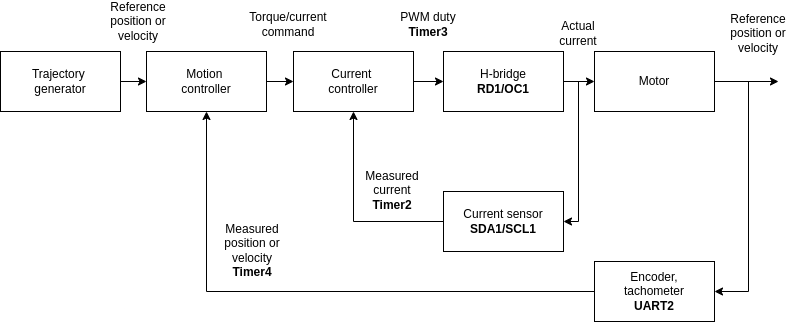
\includegraphics[width=\linewidth]{block_diagram.png}

    \pagebreak
    \item \textbf{Based on which circuit boards need to be connected to which pins of the NU32, and the
    connections of the circuit boards to the motor and encoder, sketch a proposed layout of the
    circuit boards relative to the NU32 so that wire crossing is approximately minimized. (Do
    not make a full circuit diagram at this time.)} \\

        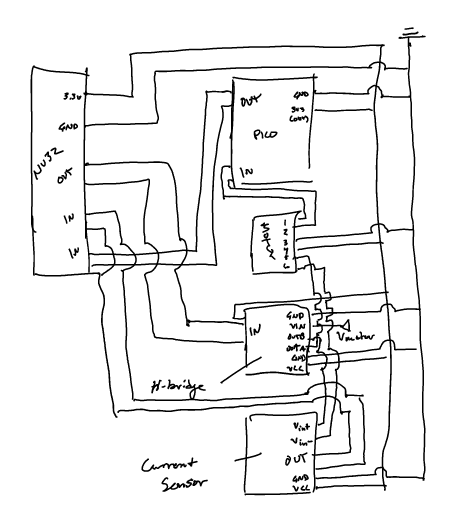
\includegraphics[width=\linewidth]{stripped_circuit.png}

    
\pagebreak
\end{enumerate}

\setcounter{section}{28}
\setcounter{subsection}{4}
\setcounter{subsubsection}{8}
\subsubsection{PWM and the H-Bridge}

\begin{enumerate}[label=\textbf{\arabic*})]
    \setcounter{enumi}{7}
    \item \textbf{Now that the PWM output appears to be working, it is time to wire up the DRV8835
    H-bridge circuit, as discussed in Chapter 27.1.1, to the motor and the PIC32 outputs
    (Figure 28.8). Notice that the 15 mohm resistor on the current-sense PCB is in series with
    the motor. Turn in a circuit diagram showing all connections of the H-bridge to the
    NU32, motor, and current sensor PCB.} \\

    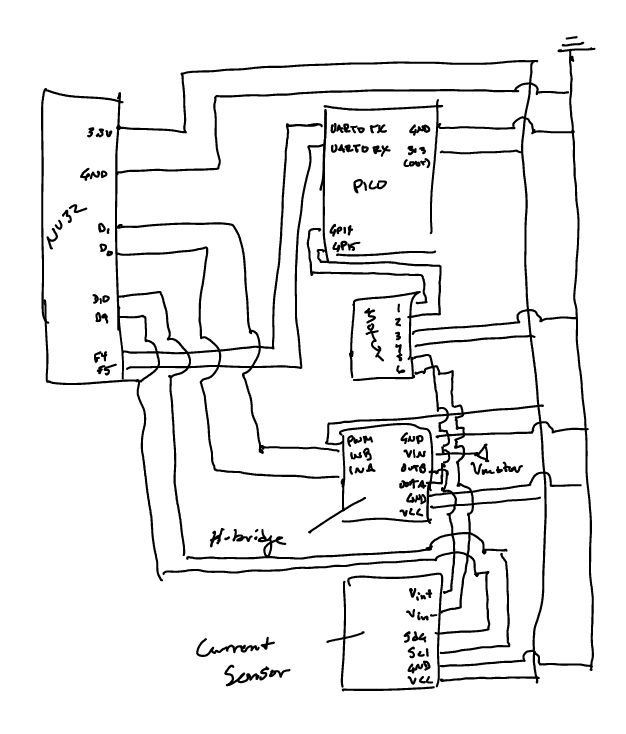
\includegraphics[width=\linewidth]{circuit_diagram.png}
\end{enumerate}



\end{document}
